\section{Technical Challenges}

\subsection{7 vs. 7}
    This competition extends the ideas from the mixed team competition, and 1 vs. 1 remote challenge from RoboCup 2021 to a standardized 7 vs. 7 on-site competition. Another goal is to enforce more collaborative game play. This challenge will only be executed if at least four teams participate.

    \subsubsection{Condition for participation} % PG
    \label{sec:7vs7:condition_for_participation}
        \begin{itemize}
            \item Teams need at least four own robots to play with. 
            \item Teams have to provide two tested robots (\textbf{only V6 version}) to a robot pool.
            \item The pool robots have to be calibrated in limited time.
        \end{itemize}

    \subsubsection{Rules}
        This challenge bases on all rules from the 5 vs. 5 competition (Sections~\ref{sec:setup_environment} — \ref{sec:judgment}). The following list contains extended and changed rules for this challenge in order to ensure, among other things, the safety of pool robots:

        \paragraph{Players}
            In total each team consists of 7 players without a substitution robot. The 7 robots consist of 4 own and 3 pool robots. Whereby the pool robots are only V6s. Each jersey shirt has therefore now player numbers between 1 and 7 printed on it (\cf Section~\ref{sec:team_markers}). Also the new positions of the initial kick-off (\cf Section~\ref{sec:initial-kick-off}) for 7 robots can be seen in Figure~\ref{fig:initial_positions_7vs7}.
            \begin{figure}[t!]
            	\begin{center}
            		\leavevmode
            		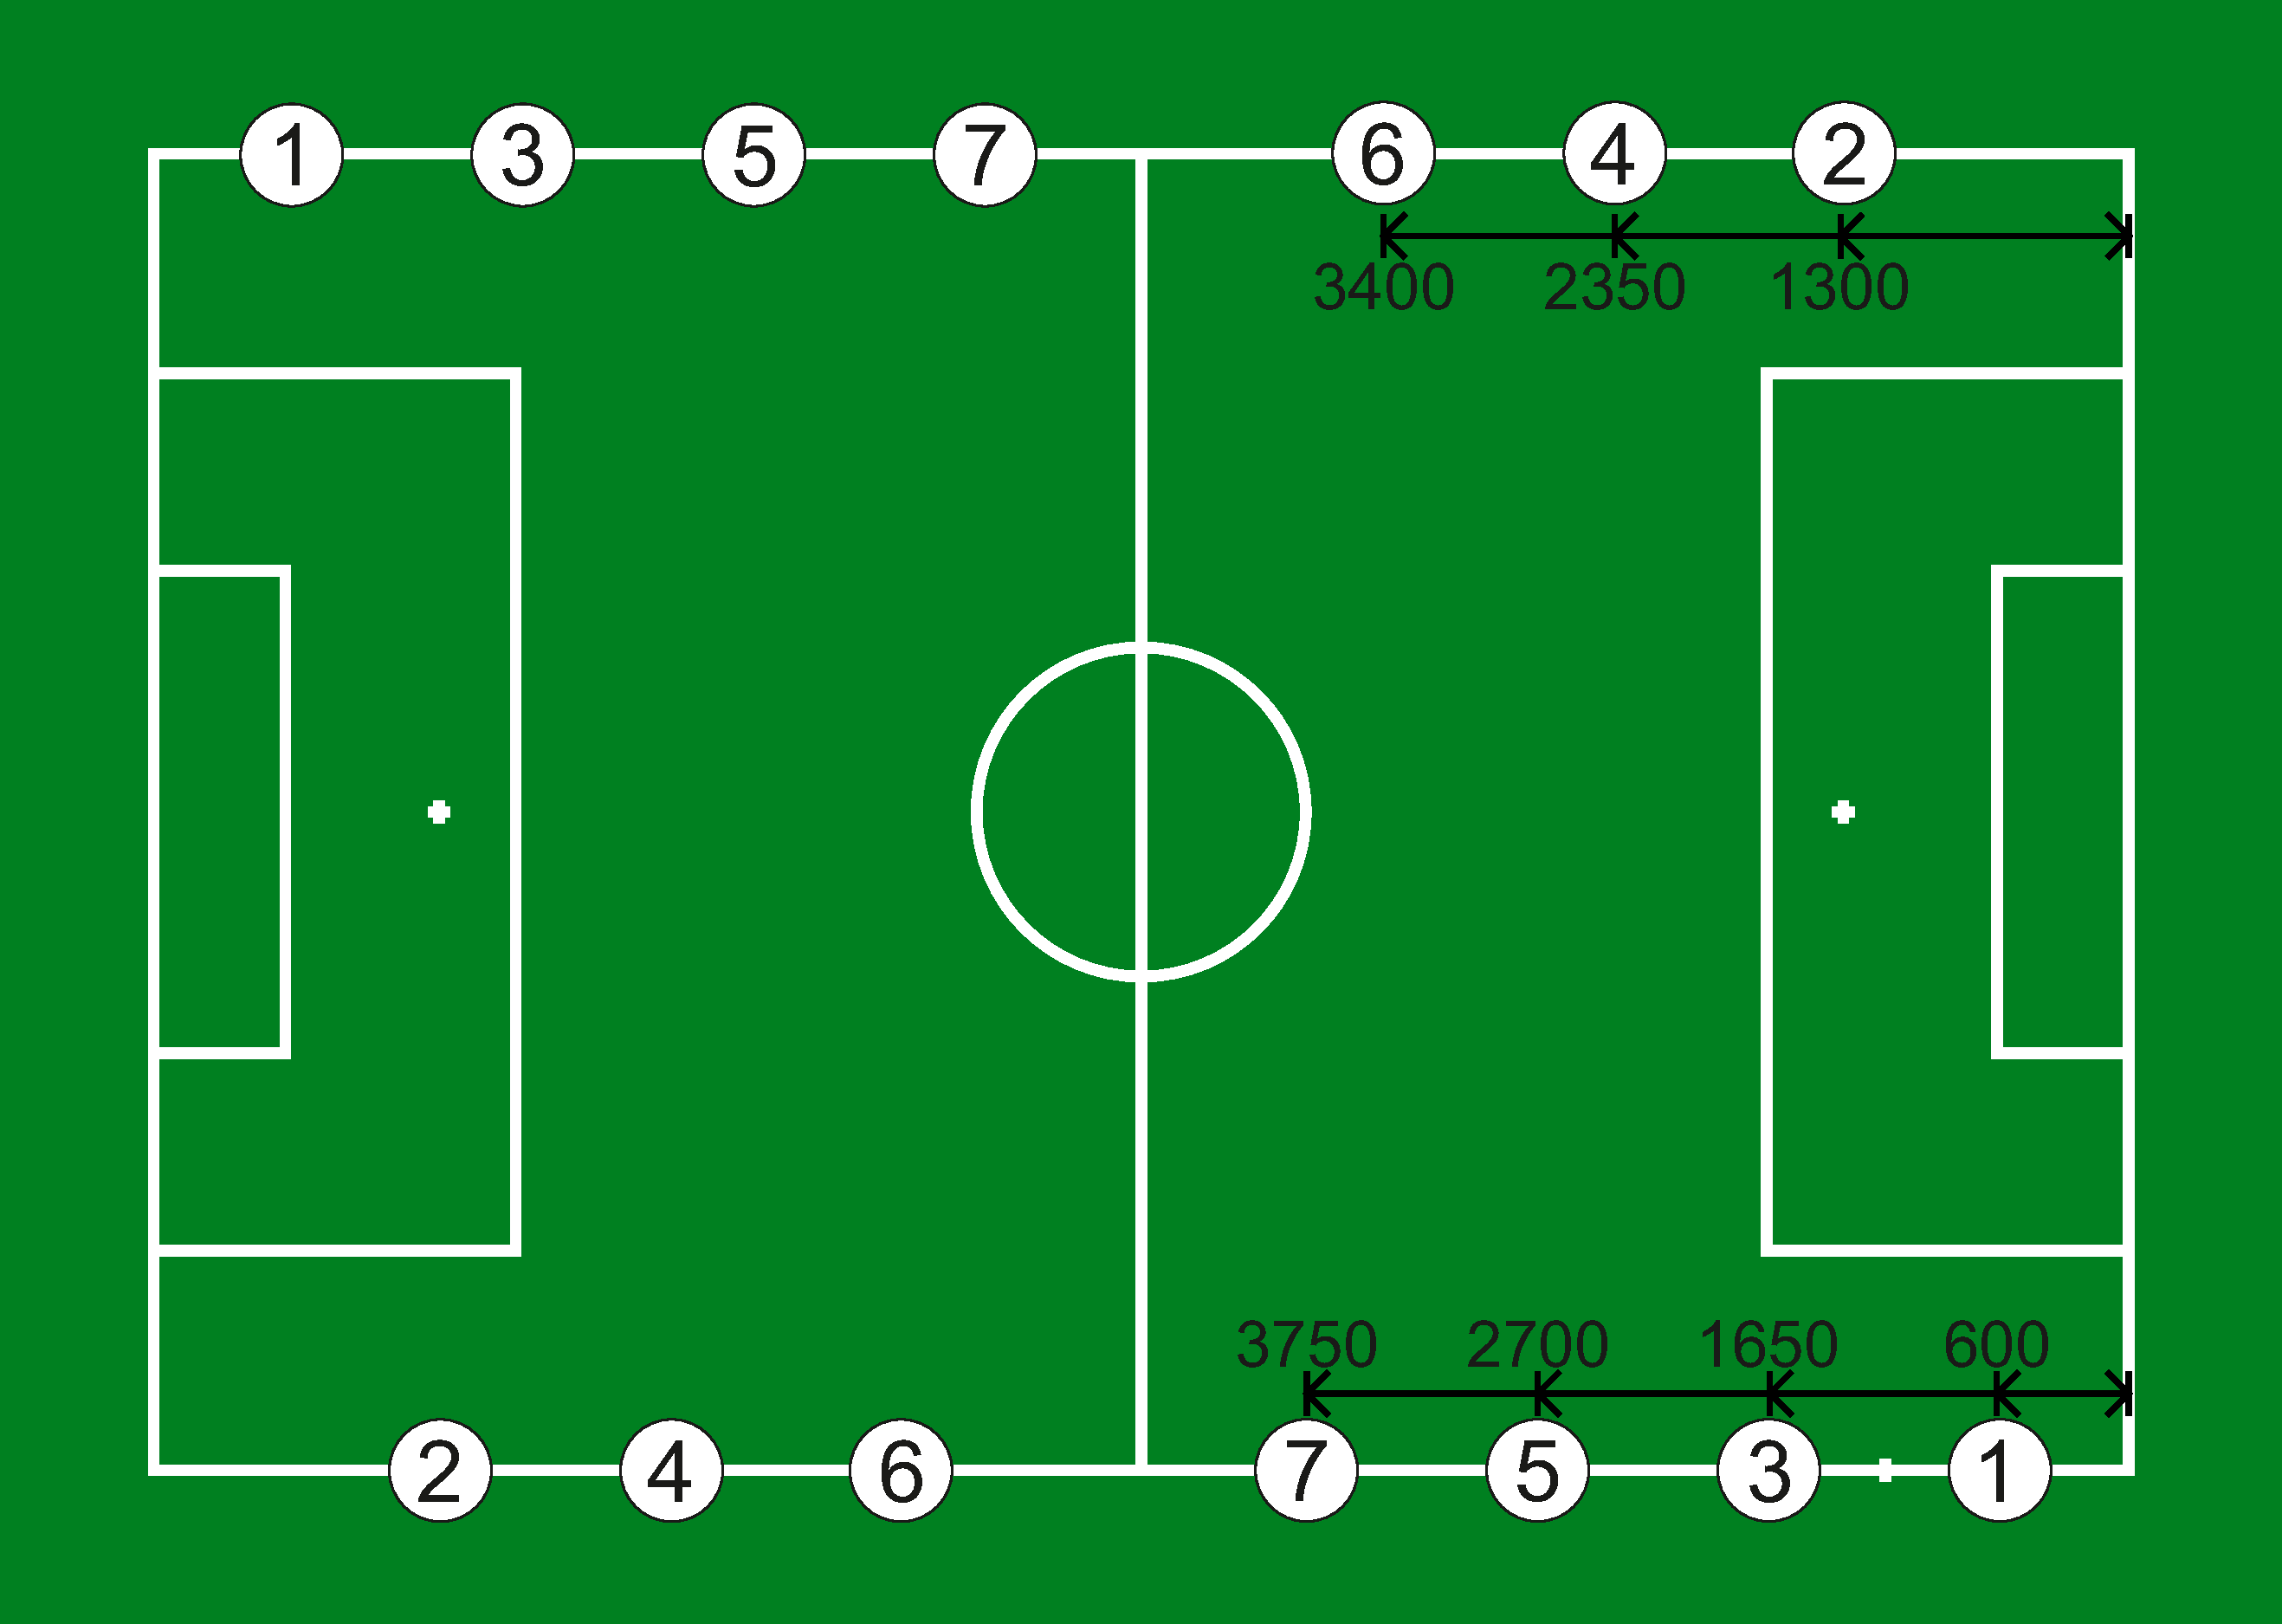
\includegraphics[width=1\columnwidth]{figs/initial_positions_7vs7.pdf}
            		\caption{Positions, player numbers and distances from the center of the goal line for the initial kick-off of the 7 vs. 7 robots.}
            		\label{fig:initial_positions_7vs7}
            	\end{center}
            \end{figure}

        \paragraph{Referees}
            \label{sec:7vs7:referee}
            All referees are allowed to prevent robots from crashing to the ground by catching them beforehand and then laying them down gently. Additionally the head referee decides whether a robot excessively damages itself and should remove it from the field via a forced “Request for Pick-up”, \cf Section~\ref{sec:request_for_pickup}.

        \paragraph{Robot Pool}
            Each team has to contribute at least 3 robots to the robot pool, \cf Section~\ref{sec:7vs7:condition_for_participation}. If a team cannot provide enough own robots and there are still functional robots in the robot pool, then this team can get more than the 3 robots from the pool to restock up to 7 robots. However, the final decision is still up to the head referee. \\
            The robot pool exists only virtually, so that there is no central location where all pool robots are stored. Each team is also allowed to use their own pool robots when they are not in use. However, each pool robot gets a unique ID and in order to be able to recognize the pool robots visually, a sticker is attached to the outer sides of the upper arms and on the back of the head. 

        \paragraph{Robot Pool Evaluation}
            In order to guarantee that the pool robots are functional and all parts are working within their limits each team has to provide a prove of functionality one hour before a specific pool robot is planned for a game. Also the team has to ensure that this robot had at least a cooldown period of \qty{15}{\minute} and is charged to at least \qty{80}{\percent} 
            A common robot evaluation image will be provided by the community with a standardized setup procedure (custom image) and with automatic calibration. Afterwards the robot should walk towards a ball and shoot it. If this evaluation is completed without any problems within a given time \todo{time} and the robot falls down less than 2 times, the evaluation is to be rated as functional. Otherwise, this robot is considered to be non-functional for the time being. Every team can propose such an image up to the \todo{deadline}, as well as additional tests which should be included in such an evaluation image.            

        \paragraph{Hardware Related Penalties}
            \label{sec:7vs7:hardware_related_penalties}
            Since teams are partially playing with robots from other teams, there is a maximum of two hardware related penalties for each robot in the first half and one more in the second half. 
            Hardware related penalties are:
            \begin{itemize}
                \item fallen robot or inactive robot, \cf Section~\ref{sec:fallenrobots}
                \item request for pick-up in the playing or ready state — either by the team or forced by the head referee, \cf Section~\ref{sec:request_for_pickup} and Section~\ref{sec:7vs7:referee}. 
            \end{itemize}
            These penalties are counted by the GameController operator and after that a robot with additional hardware related penalties is excluded for the rest of the game (they are transitioned into the unstiffed state by the assistant referees, \cf Section~\ref{sec:robot_states})!

        \paragraph{Own Pushing}
            In addition to the normal pushing rules, \cf Section~\ref{sec:player_pushing}, pushing may now occur between any robots, i.e., also between teammates.

        \paragraph{Limited Diving}
            Pool robots are not allowed to dive for the ball on purpose, \cf Section~\ref{sec:fallenrobots}, except for penalty kicks! In case of violation, the infringing robot will be taken out according to the forced ``Request for Pick-up'' rule, \cf Section~\ref{sec:7vs7:referee}, and therefore counts as a hardware related penalty, \cf Section~\ref{sec:7vs7:hardware_related_penalties}. However, this restriction does not apply to the team's own robots. 

        \begin{itemize}
            \item setup procedure % PG
            \item Modus % PG
        \end{itemize}


\subsection{Visual Referee Challenge}
    
    \subsubsection{Challenge Goal}

        For the moment robots receive the decision made by the head referee either from a short whistle or a GC message. To improve the perception of the robot and to listen more to the head referee this challenge introduces visual referee signs.

    \subsubsection{Challenge setup}

        One robot of the challenged team is placed in the center circle facing the head referee standing on the opposite T-junction to the GC. The referee wears red glows. The robot is listing and watching the referee. The general procedure is as follows:

        \begin{itemize}
            \item The referee blows the whistle.
            \item The referee shows his decision for \qty{15}{\second}.
            \item During that time or in the additional \qty{10}{\second} the robot has time to phrase the referee's decision, e.g., ```Kick-off left team'''. \todo{Or we use a TCP message}
        \end{itemize}

        This procedure will be continued for in total four times. Each time, the referee chooses a new decision.

    \subsubsection{Available Decisions}
        
        For each decision (not all, because some decisions have to be shown on place, e.g., throw in) will be described and pictured.

        \begin{itemize}
            \item \textbf{Kick-Off} 
            \begin{figure}[ht!]
                
\includegraphics{figs/kick-off_referee.jpg}
            \end{figure}
        \end{itemize}

    \subsubsection{Challenge evaluation}
        The time from the whistle until the robots starts messaging will be counted for each run.
        For each decision two points can be awarded: One for the right decision itself and one for the right team awarded to or against.
        The ranking is based on the sum of points. Higher number of points leads to a higher ranking. For teams with equal points the sum of the runs will be used. Less time used leads to a higher ranking.
        

\subsection{Dynamic Ball handling}

    This challenge extends the idea of RoboCup 2021's Passing Challenge. The purpose of this challenge is to enhance skills in ball passing and handling, and in robot's movement estimation.

    \subsubsection{Challenge Goal}

    Score as attacking team a goal after a double pass without letting the opponents players touch the ball.

    \subsubsection{Challenge Setup}

    This challenge uses a standard SPL field, with GameController and 3 attacking robots provided by the challenged team and three defending robots operating with a provided common image from another team.\todo{Attacking team's robots will be defender next round} A common image will be provided by the community with the standardized setup procedure and with automatic calibration. Every team can propose such an image \todo{deadline}. The image will be tested if they match the requirements. \todo{Was wird getestet} If more than one exists, than multiple images will be provided and for each run a new one will be randomly selected.
    \todo{Criterias for images, how to setup}

    \todo{Drawing of setup and variance}

    The robots are placed by the referees with some randomness as follows:
    \begin{itemize}
        \item \textbf{Attacker:} 1st goal box front line; 2nd next to center line left of center circle; 3rd next to center line right of center circle
        \item \textbf{Defender:} 1st within center circle; 2nd front line penalty box; 3rd goalkeeper in the middle between the two goal posts.
        \item \textbf{Ball:} On penalty spot of the attacking team's side 
    \end{itemize}

    Each team has three attempts to run this challenge.

    \subsubsection{Challenge Execution}

    All six robots have to be in the Wi-Fi. In initial the robots get placed at their randomized starting positions. GC goes from ready directly into set. The ball gets placed, and the head referee starts the challenge execution with one whistle, like at kick-off. If a robot does not listen to the whistle, it will get the delayed playing signal from the GC.

    In playing the following happens: The 1st attacker plays the ball towards the 2nd or 3rd attacker will he is under attack by the 1st defender. A pass counts as a valid pass if the ball stops in front of the receiving robot towards the opponent's goal. The ball has to stop in the vicinity of the receiving robot (at max \qty{1}{\metre} distance between receiver and ball). \todo{Visualization}
    The 1st defender does not walk back in its own half. The objective of the defending team is to intercept the passes, see stopping criteria.
    \todo{3rd defender, remains within goal box}
    \todo{Make clear, attacking defending robot, defending defing robot, goalie}
    \todo{Limit max speed of Defenders}

    After the 2nd or 3rd attacker received the ball, and the ball is in the defender's half, it gets attacked by the 2nd defender. The task of the 2nd or 3rd attacker is now to pass towards the 3rd or 2nd attacking robot, which than shots onto the goal. \todo{Goalkeeper disallow dive; Where to move; only on the line}

    \subsubsection{Challenge Scoring}\todo{Rephrase this}

    The challenge execution will be stopped, when one of the following events occur:

    \begin{itemize}
        \item A defender touches the ball.
        \item Ball leaves the field.
        \item An attacker pushes.
        \item The execution duration exceeds \qty{3}{\minute}.
        \item A goal scored with zero or one pass.
    \end{itemize}

    A score for the run will be calculated based on the following rules:

    The time in seconds in playing counts. Passing a ball in the back of a receiver adds 10 extra seconds each time. Scoring a goal after two passes subtracts 30 seconds.
    If the ball left within the goal box the field, or it got intercepted by goalkeeper (both after 2 passes) the time counts.
    If the execution gets stopped, the for the run a time of 180 seconds is taken.

    The final result is the mean time out of three runs.

\subsection{Video analysis / statistics}
\begin{itemize}
    \item Statistics needed to evaluate the progress of the league.
    \item Only GameController statistics are not sufficient for this.
    \item Create video statistics like in real soccer games.
\end{itemize}

    \subsubsection{Challenge Goal}
    \begin{itemize}
        \item Long Term: Create Online/Offline Game Statistics from a go-pro type camera viewpoint. E.g. time under control, shots on goal, passes, ... .
        \item Short Term: Calculate the extrinsic camera parameters (camera matrix) and locate/track all moving objects (ball, robots) on the field.
        \item Designed as open challenge: Teams show a small presentation/poster of their approach, with the team leaders then voting afterwards to determine the winners.
    \end{itemize}

    \subsubsection{Condition for participation}
        \begin{itemize}
            \item Express the interest to participate in this challenge by 2021-12-31.
            \item Label an assigned video, from the RC2019, until 2022-02-01 \todo{date} in order to form a shared ground truth database.
            \item Implementation of the own approach in order to achieve the short term or the long term goal, or only parts of it.
            \item Prepare a poster and a short 5-10 minutes presentation for the RC2022 showing the results of your approach.
        \end{itemize}
    
    \subsubsection{Labeling}
        Input data:
        \begin{itemize}
            \item Get the assigned go-pro videos from a game of the RC2019.
            \item Additionally you get the GC data, TeamCom logs and the intrinsic calibration of the go-pro.
        \end{itemize}

        Output data:
        \begin{itemize}
            \item Calculate the extrinsic camera parameters (camera matrix). Preferably for each frame, although this is mainly necessary when the camera was moved/wobbled. However, it should be checked at least once for each minute whether the camera matrix is still appropriate.
            \item Label all robots and the (main) ball: These objects should be labeled using bounding boxes. Special attention should be paid to the bottom edge as this will be used to determine the position of the object.
            \item In addition, the robots must be labeled with their jersey color and number.
            \item Send the ground truth data in a common format \todo{which one?} to the TC until 2022-02-01.
            \item The TC will then publicly upload this data to form a shared ground truth database. 
        \end{itemize}